%%%%%%%%%%%%%%%%%%%%%%%%%%%%%%%%%%%%%%%%%%%%%%%%%%%%%%%%%%%%%%%%%%%%%%%%%%%%%%%%%%%%%%%%%%%%%%%%%%%%%%%%%%%%%%%%%%%%%%%%%%%%%%%%%%%%%%%%%%%%%%%%%%%%%%%%%%%%%%%%%%%
% Written By Michael Brodskiy
% Class: Fundamentals of Networks
% Professor: E. Bernal Mor
%%%%%%%%%%%%%%%%%%%%%%%%%%%%%%%%%%%%%%%%%%%%%%%%%%%%%%%%%%%%%%%%%%%%%%%%%%%%%%%%%%%%%%%%%%%%%%%%%%%%%%%%%%%%%%%%%%%%%%%%%%%%%%%%%%%%%%%%%%%%%%%%%%%%%%%%%%%%%%%%%%%

\documentclass[12pt]{article} 
\usepackage{alphalph}
\usepackage[utf8]{inputenc}
\usepackage[russian,english]{babel}
\usepackage{titling}
\usepackage{amsmath}
\usepackage{graphicx}
\usepackage{enumitem}
\usepackage{amssymb}
\usepackage[super]{nth}
\usepackage{everysel}
\usepackage{ragged2e}
\usepackage{geometry}
\usepackage{multicol}
\usepackage{fancyhdr}
\usepackage{cancel}
\usepackage{siunitx}
\usepackage{physics}
\usepackage{tikz}
\usepackage{mathdots}
\usepackage{yhmath}
\usepackage{cancel}
\usepackage{color}
\usepackage{array}
\usepackage{multirow}
\usepackage{gensymb}
\usepackage{tabularx}
\usepackage{extarrows}
\usepackage{booktabs}
\usepackage{lastpage}
\usepackage{float}
\usetikzlibrary{fadings}
\usetikzlibrary{patterns}
\usetikzlibrary{shadows.blur}
\usetikzlibrary{shapes}

\geometry{top=1.0in,bottom=1.0in,left=1.0in,right=1.0in}
\newcommand{\subtitle}[1]{%
  \posttitle{%
    \par\end{center}
    \begin{center}\large#1\end{center}
    \vskip0.5em}%

}
\usepackage{hyperref}
\hypersetup{
colorlinks=true,
linkcolor=blue,
filecolor=magenta,      
urlcolor=blue,
citecolor=blue,
}


\title{Conceptual Homework 2}
\date{October 23, 2023}
\author{Michael Brodskiy\\ \small Professor: E. Bernal Mor}

\begin{document}

\maketitle

\begin{enumerate}

  \item Do routers have IP addresses? If so, how many? If not, why?

    Yes, routers have IP addresses. The exact number depends on the router and network configuration; however, we know that there are, at the very least, two addresses. This is due to the fact that a router must have an incoming address and an outgoing address that it must differentiate between. There is no absolute maximum amount for the amount of addresses a router may have, but there are many factors which can limit it, such as: quantity of allocated addresses to a network and hardware of a router (CPU, RAM, etc.).

  \item Suppose an application generates chunks of 960 bytes of data, and each chunk gets encapsulated in a TCP segment and then an IPv4 packet (no optional header fields). What percentage of each packet will be overhead (including transport and network layer), and what percentage will be application data?

    Given that there are no optional header fields, we know that the length of the TCP segment = length of the IP segment = 20 bytes. Thus, we can calculate the total segment size:

    $$s_{tot}=960+20+20$$
    $$s_{tot}=1000[\text{bytes}]$$

    We can then find the respective percents as:

    $$\%_{data}=\frac{960}{1000}$$
    $$\boxed{\%_{data}=96\%}$$
    $$\%_{head}=\frac{40}{1000}$$
    $$\boxed{\%_{head}=4\%}$$

  \item Suppose a router has four links, numbered 0 through 3. Destination-based forwarded is used and the forwarding table is given by:

    \begin{center}
      \begin{tabular}[h!]{|c|c|c|}
        \hline
        Entry & Destination Address & Output Link Interface\\
        \hline
        1 & 11100000 00****** ******** ******** & 0\\
        \hline
        2 & 11100000 01000000 ******** ******** & 1\\
        \hline
        3 & 1110000* ******** ******** ******** & 2\\
        \hline
        4 & 11100001 1******* ******** ******** & 3\\
        \hline
        5 & Otherwise & 4\\
        \hline
      \end{tabular}
    \end{center}

  Obtain the appropriate output link interface for the datagrams with the following destination addresses. \underline{Explain how you reached your answer and include the interface and} \underline{the table entry chosen}

  First and foremost, we need to find which address range each of the above corresponds to. We begin by converting to decimal:

  $$\text{Entry 1: } 11100000\, 00000000\, 00000000\, 00000000\text{ to }11100000\, 00111111\, 11111111\, 11111111$$
  $$\text{Entry 1: } 224.0.0.0\longleftrightarrow 224.63.255.255$$
  $$\text{Entry 2: } 11100000\, 01000000\, 00000000\, 00000000\text{ to }11100000\, 01000000\, 11111111\, 11111111$$
  $$\text{Entry 2: } 224.64.0.0\longleftrightarrow224.64.255.255$$
  $$\text{Entry 3: } 11100000\, 00000000\, 00000000\, 00000000\text{ to }11100001\, 11111111\, 11111111\, 11111111$$
  $$\text{Entry 3: } 224.0.0.0\longleftrightarrow225.255.255.255$$
  $$\text{Entry 4: } 11100001\, 10000000\, 00000000\, 00000000\text{ to }11100001\, 11111111\, 11111111\, 11111111$$
  $$\text{Entry 4: } 225.128.0.0\longleftrightarrow225.255.255.255$$

    \begin{enumerate}

      \item 11001000 10010001 01010001 10101010 

        Again, we begin by converting this to decimal notation:

        $$11001000\, 10010001\, 01010001\, 10101010\longrightarrow 200.145.81.170$$

        This address is not in any of the given ranges, so it is sent to \underline{entry 5,}\\ \underline{destination: Otherwise, output link interface 4}.

      \item 11100001 01000000 11000011 00111100 

        Converting this to decimal notation:

        $$11100001\, 01000000\, 11000011\, 00111100\longrightarrow 225.64.195.60$$

        We can see that this datagram matches with output link 2 (entry 3); thus, this packet will go to \underline{entry 3, destination: 1110000* ******** ******** ********,}\\\underline{output link interface 2}

      \item 11100001 10000000 00010001 01110111

        Converting this to decimal notation:

        $$11100001\, 10000000\, 00010001\, 01110111\longrightarrow 225.128.17.119$$

        Again, though this datagram may be found in the ranges for output link interfaces 2 and 3 (entries 3 and 4), we know that, based on longest prefix matching, the packet must go to \underline{entry 4, destination: 11100001 1******* ******** ********,}\\\underline{output link interface 3}

      \item 11100000 01000000 11001100 00011101

        Converting this to decimal notation:

        $$11100000\, 01000000\, 11001100\, 00011101\longrightarrow 224.64.204.29$$

        Though this address fits into the ranges of output links of 1 and 2 (entries 2 and 3), because of longest prefix matching, the packet will be sent to \underline{entry 2, destination:}\\\underline{1110000 01000000 ******** ********, output link interface 1}

    \end{enumerate}

  \item What is a private network address? Should a datagram with a private network address ever be present in the larger public Internet? Explain.

    A private network address has a function similar to public addresses, except that it exists only in the ``intra-net'' (internal to the network). As such, a private address is only useful to devices within the same local network. In this manner, a datagram with a private network address should never exist within the public Internet. Furthermore, in the event that a datagram with a private network address would somehow end up in the Internet (which is not possible), there may be many problems as the private network address may be used in other private networks.

  \item

    \begin{enumerate}

      \item What is meant by a control plane that is based on per-router control? Are the data plane and the control planes implemented within the same devices? Briefly explain your answer.

        If the control plane is based on per-router control, this essentially means that each router individually must control its own traffic. Such a system is generally implemented in large networks, as each router can make informed decisions about how to operate within the large network. This allows routers to optimize their traffic flow based on their condition. A downside, however, is that allowing each router to decide individually may lead to inefficiencies in the grand scheme of things. In the case of per-router control, the data and control planes are generally implemented within the same devices, as there is no centralized entity to control either plane.

      \item What is meant by a control plane that is based on logically centralized control? Are the data plane and the control planes implemented within the same devices? Briefly explain your answer

        A control plane that is logically centralized means that there is a single entity computing and distributing forwarding tables to routers in a network. Each router obtains its forwarding tables by interacting with the centralized entity. Such an approach is common for software-defined networking (SDN). In this case, the control plane is implemented by the logical controller, while the data plane remains at the per-router level.
        
    \end{enumerate}

  \item Consider the following network. With the indicated link costs, use Dijkstra’s algorithm to compute the least-cost path from $x$ to all network nodes and then obtain \underline{the resulting forwarding table}. Show how the algorithm works by \underline{computing a table }\\\underline{similar to the tables we have seen in class}.

    \begin{figure}[H]
      \centering
      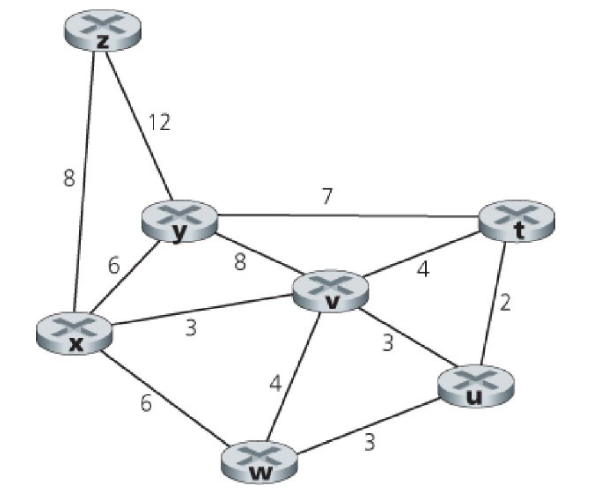
\includegraphics[width=.6\textwidth]{Figures/Djikstra.png}
      \caption{Figure for Problem 6}
      \label{fig:1}
    \end{figure}

    We can begin by constructing a table from $x$ to perform Dijkstra's algorithm:

    \begin{center}
      \begin{tabular}[h]{|c|c|c|c|c|c|c|c|c|}
        \hline
        Step & $N'$ & $D/p(t)$ & $D/p(u)$ & $D/p(v)$ & $D/p(w)$ & $D/p(x)$ & $D/p(y)$ & $D/p(z)$\\
        \hline
        0 & $x$ & $\infty$ & $\infty$ & $3,x$ & $6,x$ & $\bold{0,x}$ & $6,x$ & $8,x$\\
        \hline
        1 & $xv$ & $7,v$ & $6,v$ & $\bold{3,x}$ & $6,x$ & & $6,x$ & $8,x$\\
        \hline
        2 & $xvu$ & $7,v$ & $\bold{6,v}$ & & $6,x$ & & $6,x$ & $8,x$\\
        \hline
        3 & $xvuw$ & $7,v$ & & & $\bold{6,x}$ & & $6,x$ & $8,x$\\
        \hline
        4 & $xvuwy$ & $7,v$ & & & & & $\bold{6,x}$ & $8,x$\\
        \hline
        5 & $xvuwyt$ & $\bold{7,v}$ & & & & & & $8,x$\\
        \hline
        6 & $xvuwytz$ & & & & & & & $\bold{8,x}$\\
        \hline
      \end{tabular}
    \end{center}

    To summarize the data, we construct a different table:

    \begin{center}
      \begin{tabular}[h]{|c|c|c|c|c|c|c|}
        \hline
        Edge & $x\to t$ & $x\to u$ & $x\to v$ & $x\to w$ & $x\to y$ & $x\to z$ \\
        \hline
        Path & $xvt$ & $xvu$ & $xv$ & $xw$ & $xy$ & $xz$\\
        \hline
        Cost & $7$ & $6$ & $3$ & $6$ & $6$ & $8$\\
        \hline
      \end{tabular}
    \end{center}

    From here, we can construct a least cost tree:

    \begin{figure}[H]
      \centering
      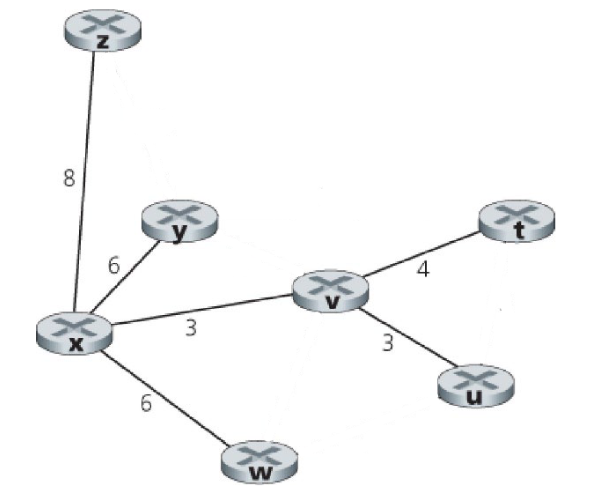
\includegraphics[width=.6\textwidth]{Figures/LeastTree.png}
      \caption{Least Cost Tree}
      \label{fig:2}
    \end{figure}

    Finally, we can construct a forwarding table (from $x$):

    \begin{center}
      \begin{tabular}[h]{|c|c|c|c|c|c|c|}
        \hline
        Destination: & $t$ & $u$ & $v$ & $w$ & $y$ & $z$\\
        \hline
        Outgoing Link: & $(x,v)$ & $(x,v)$ & $(x,v)$ & $(x,w)$ & $(x,y)$ & $(x,z)$ \\
        \hline
      \end{tabular}
    \end{center}

\end{enumerate}

\end{document}

